% !TEX program = lualatex
% !BIB program = biber
\documentclass[12pt]{iopart}
\usepackage[T1]{fontenc}
\usepackage[utf8]{inputenc}
\usepackage{amssymb}
\usepackage{amsbsy}
\usepackage{graphicx}
\usepackage{color}
\usepackage{subfig}
\usepackage{wasysym}
\graphicspath{{../imgs/}}
% Begin Reference Packages and additions
\usepackage[
backend=biber,
style=authoryear-icomp,
firstinits=true,
doi=false,
isbn=false,
url=false,
citestyle=authoryear,
maxbibnames=9,
maxcitenames=1,
uniquename=false,
uniquelist=false
]{biblatex}
\renewbibmacro*{name:andothers}{% Based on name:andothers from biblatex.def
  \ifboolexpr{
    test {\ifnumequal{\value{listcount}}{\value{liststop}}}
    and
    test \ifmorenames
  }
    {\ifnumgreater{\value{liststop}}{1}
       {\finalandcomma}
       {}%
     \andothersdelim\bibstring[\emph]{andothers}}
    {}}
\addbibresource{refs.bib}
\newcommand{\citeauthorandyear}[2][]{
   \citeauthor{#2} (\citeyear[#1]{#2})}
% End reference packages
\usepackage{multirow}
\usepackage{tikz}
\newcommand{\VB}{{\mbox{\bf V}}}
\newcommand{\YB}{{\mbox{\bf Y}}}
\newcommand{\CB}{{\mbox{\bf C}}}
\newcommand{\JB}{{\mbox{\bf J}}} 
\newcommand{\vB}{{\mbox{\bf v}}}
\newcommand{\COMMENT}[1]{ \textsf{\color{blue}{{COMMENT: #1}}} }
%\graphicspath{{../images/}}
\begin{document}

\title{%
FEM mesh refinement for 3D Electrical Impedance Tomography % Enough acronyms?
}

 \author{%
Symon Stowe$^{1*}$,
Bart\l{}omiej Grychtol$^2$,
Andy Adler$^1$}

\address{
$^1$Systems and Computer Engineering, Carleton University, Ottawa, Canada
$^2$OTHER
}
\ead{*Corresponding author: Email: symonstowe@sce.carleton.ca}
\vspace{10pt}

\begin{abstract}

\end{abstract}

\section{Introduction}

Electrical Impedance Tomography (EIT) reconstructs images of 
electrical tissue properties within a body from electrical
transfer impedance measurements at surface electrodes. For
biomedical imaging applications, it is being actively studied
for monitoring
the movement of air and blood in the thorax, and for imaging
the head and breast. Reconstruction of EIT images requires
the solution of an inverse problem in soft field tomography.
EIT imaging requires an iterative solution in which, at each step,
a sensitivity matrix, $\bf J$, of
the relationship between internal changes and measurements
is calculated, and then a pseudo-inverse of $\bf J$ is used
to update the image estimate. (Several algorithms use
one step of the iterative solution~\parencite{lionheart_eit_2004}.)
EIT image reconstruction is ill-posed, since the physics of
current propagation imply that sensitivity is largest near
the electrodes and smallest in the body center.

It is therefore clear that a precise  calculation of $\bf J$ is
required for solution accuracy. Since it is generally not
possible to use analytic solutions (because of the non-regular
shapes of biological bodies and the boundary conditions on a
conductive electrode) the finite element method (FEM) is typically
used. 
One key advantage of FEM is that element size can be
selectively refined in regions to meet solution accuracy. 
The FEM solution will be more accurate as more elements are
added so a high mesh density is often desired to achieve an 
accurate solution. In EIT the sensitivity is not uniform 
across the entire model.
Thus
it has generally been recommended in the EIT literature 
that FEMs be refined near electrodes, since the electric
field and sensitivity is largest there. 
This recommendation gives rise to several questions: 
1) No thorough analysis has been made to determine how much 
refinement is required. Given an ``FEM element budget", how
much should be ``spent" on elements near electrodes relative to 
the body core?
2) How can mesh refinement be controlled more precisely 
to refine FEM electrodes on arbitrary
body shapes? 
3) How do different freely available meshing tools that are
commonly used with EIT compare when used to refine 3D meshes?

Previously with EIT, mesh refinement has primarily been either 
constant, or based on 
the complexity of geometric features
and gradients between different volumes and surfaces~\parencite{grychtol_fem_2013}.  
Netgen~\parencite{schoberl_netgen_1997} and Gmsh~\parencite{geuzaine_gmsh_2009} have been used alongside 
EIDORS~\parencite{adler_uses_2006} to generate meshes in both 2D and 3D. 
Currently refinement around electrodes is most frequently performed by 
setting a mesh density for the electrodes and allowing the mesh density to 
decay towards the maximum mesh size. This does not allow the user to specify 
the rate of decay or precisely control the mesh size in regions nearest to 
the  electrodes where sensitivity to change is highest.

A FEM that accurately represents the anatomy of the imaged region 
can greatly increase the quality of the reconstructed image~\parencite{grychtol_impact_2012},
but increasing the complexity of mesh surfaces presents additional challenges for
mesh refinement. Using EIDORS in ,  electrodes can be placed on the surface of complex boundaries in 
EIDORS~\parencite{grychtol_fem_2013}, but the current functionality does not allow the
refinement around the electrodes to be controlled, or for users to specify internal 
refinement and structures.
Most commercially available FEM packages
do not conveniently provide such capability either.

%Due to the increasing number of options for implementing mesh refinement around the
%electrodes it is also important to consider which gives the highest quality mesh. 
%The quality of a mesh dictates the accuracy of the subsequent analysis 
%and solution, and can be characterized by the properties of the tetrahedra
%comprising the model~\parencite{Parthasarathy1993}.

In this paper we present a comparison between Gmsh and 
Netgen based mesh refinement around electrodes and structures, and evaluate the 
effect of mesh refinement techniques on error in  the sensitivity matrix, 
$\bf J$. 
We also present a tool for mesh refinement around both external and internal
electrodes and geometric structures in EIDORS. 

\section{METHODS}
\subsection{Overview}
A cylinder ($\diameter=0.5$~m, height $h=0.25$~m) with four square electrodes 
(5~cm edge length) placed equidistantly around the perimeter at mid-height was
meshed with Netgen (version 5.3.1)~\parencite{schoberl_netgen_1997} and Gmsh 
(version 4.7.0)~\parencite{geuzaine_gmsh_2009}
meshing softwares.
Current was injected between adjacent electrodes and the voltage was measured between the remaining
two electrodes.
For 3D meshes an initial analysis was done building on work from 
Grychtol and Adler~\parencite{grychtol_fem_2013} where mesh density was
set by specifying the maximum edge lengths permitted on electrode surfaces
and in the volume of the FEM.
Results were compared against those generated using ultra-fine meshes. 
Calculations were performed with EIDORS (version 3.10)~\parencite{adler_uses_2006} 
in Matlab 2019b
(The Mathworks, Natick, MA, USA).


\subsection{Mesh Generation}
Meshes of different size were generated with Netgen and Gmsh by manipulating the desired
maximum edge length (maxh parameter) for the entire domain and the electrodes.
Two different mesh analyses were performed. For the first
mesh maximum element lengths were
chosen such as to divide the electrode side of 5~cm into an integer number of
segments of equal size. 
The maximum mesh element length ranged from 1 to 7 subdivisions of the electrode 
edge, while the maximum mesh element length in the ultra-fine reference mesh  
was 15 subdivisions per 
electrode edge. 
Two types of models were generated this way. Constant models C1--C7, where the mesh size 
was constant, and refined models R1--R7 where the electrode mesh size was specified and 
dissipated towards an internal mesh element size of 5cm. The numeric value in the mesh 
ID indicated the number of subdivisions per electrode edge. 
In Netgen the mesh decay was not controllable, but in Gmsh the size was set 
to increase evenly from the surface of the electrode to the centre of the model.
Figure~\ref{fig:sample_meshes} shows example meshes of coarse, fine, and refined
meshes. Figure~\ref{fig:electrode_mesh_size} shows the generated mesh structure for 
constant refinement meshes around the electrode 
for both Netgen and Gmsh. 

\begin{figure}
   \includegraphics[width=\columnwidth]{sample_meshes.pdf}
   \caption{\label{fig:sample_meshes} Sample meshes generated with Netgen (top row)
   and Gmsh (bottom row). From left to right there is: (C1) the coarsest constant
   mesh; (C5) a refined constant mesh; and (R5) a refined mesh with the same
   electrode mesh density as C5 but lower internal mesh density.}
\end{figure}

\begin{figure}
  \includegraphics[width=\columnwidth]{electrode_mesh_size.pdf}
  \caption{\label{fig:electrode_mesh_size} A view of the electrode meshing for all constant-density meshes 
  in Netgen (top row) and Gmsh (bottom row). The figure shows all electrode faces and immediate surrounding
  surroundings from coarsest (C1) to finest (C7). C represents the constant mesh refinement and the number
  represents the specified mesh subdivisions per electrode edge. The reference mesh is equivalent to C15.}
\end{figure}

For the second analysis the distribution of nodes within the 
model was changed without altering 
the total number of nodes. 
Starting with the constant mesh C3, the maximum mesh element 
length on the electrode was decreased by 10\% and the maximum mesh size in the center was
increased so that the total number of elements in the mesh was  within 10\% of the 
original mesh. 
In Netgen the mesh dissipation rate was not further controlled, and in Gmsh the mesh density 
decreased evenly from the electrode surface to the center of the model. 
To compare these meshes a section of the model was selected
encompassing all points between the center of the model and a selected electrode face.
The average 
distance, or balance point, along the x axis of the selected points was expressed 
as a percentage of the tank radius.
This process is illustrated in Figure~\ref{fig:balanceMethods}.
 
\begin{figure}
  \includegraphics[width=\columnwidth]{balance_methods.pdf}
  \caption{\label{fig:balanceMethods} A sketch of the process to determine the 
  balance point of generated meshes. A) the starting mesh; B) nodes between the
  electrode surface and the center of the model are identified; C) the 
  balance point of the nodes along the x-axis is calculated and indicated 
  by the red plane; D) a histogram showing an example distribution and balance point (red)
  for the selected model.}
\end{figure}


%The difference in meshing algorithms meant that the meshes did not have the same number
%of elements, or elements per electrode for a given input. To compare meshing 
%algorithms the error and sensitivity were compared to the average number of mesh elements\
%across all electrodes. 
%
%
%%The settings used to generate all thirty meshes and their sizes are reported
%%in Table~\ref{tab:meshes}. 
%%{\COMMENT{Broke table with new analysis - need to re-insert after electrode mesh fix.}}
%
%The mesh quality was measured as a function of the minimum angle of the tetrahedra
%for the volumetric mesh, and the minimum angle of the triangles in the surface mesh.

\subsection{Simulation}
The potential at each node \VB\ of the mesh was calculated using the finite
element method (FEM) using the linearization 
\begin{equation}
\VB = \YB^{-1}\CB
\end{equation}
where \YB\ is the admittance matrix of the FEM (and a function of conductivity
distribution) and \CB\ is a matrix representing the current injection pattern,
such that \CB$_{ij}$ represents the current injected in electrode $i$ during
the $j$-th stimulation. Here, we drive current of 1~A between two adjacent
electrodes in a single stimulation, so $C = [0\,|\,0\,|\,1\,|\,-1]^T$. 
We pick a node in the center of the FEM as ground, since it is necessary to
assume the potential on
one node for \YB\ to be invertible~\parencite{Adler1996a}.
We use the complete electrode model and assume contact impedance of
0.01~$\Omega$ in the calculation of the admittance
matrix~\parencite{polydorides_electrode_2002}. 

%The resultant potential distribution in the
%electrode plane, calculated for the finest mesh and subsequently projected onto
%a $512\times512$ pixel grid, is presented in Fig.~\ref{fig:ref:a}.
%The potential distribution \VB\ is used to visualize the current flow
%around the measuring electrodes.
% NOT CURRENTLY LOOKING AT THE CURRENT FLOW! seems to be a repeat of the same stuff

We calculate the sensitivity (or Jacobian) matrix \JB\ of measurements \vB\ to
changes in the conductivity $\sigma$ of individual elements as
$\JB_{ij}=\frac{\partial v_j}{\partial \sigma_i}$ using the adjoint
method~\parencite{polydorides_electrode_2002}. Again, since we only have one measurement, \JB\
is in fact a vector.
We construct a sensitivity image by assigning each element
$i$ of the FEM the value of \JB$_i$ divided by the element's volume.
Mean sensitivity in the plane of electrodes is then calculated by averaging
the sensitivity in fifteen planes parallel to the plane of electrodes and
spanning the height of 5~cm. Results for the finest model are presented in 
The sensitivity was projected onto a $512\times512$ array and divided into regions
of interest for the center (C), at the electrode (E) and between the center and electrode
(M). The resulting sensitivity for the reference mesh calculated with Gmsh and the 
selected regions of interest is presented in Figure~\ref{fig:roiMethods}.

\begin{figure}
  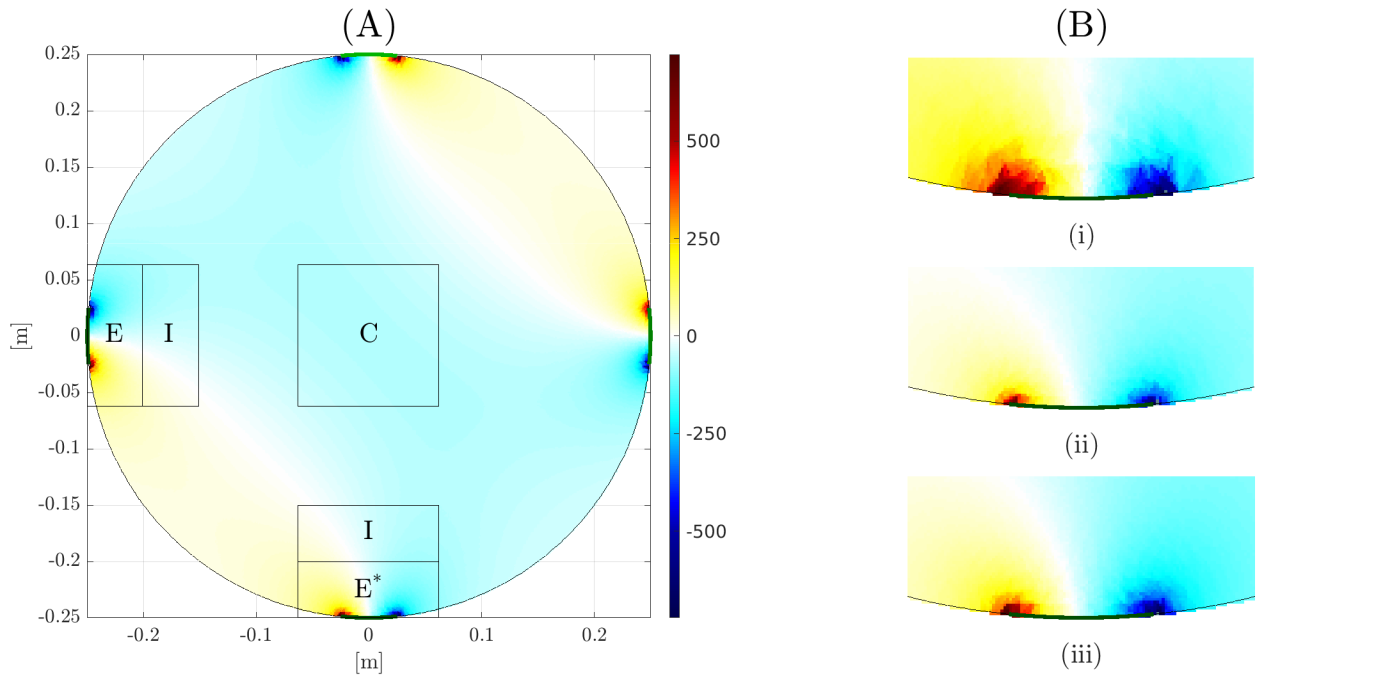
\includegraphics[width=\columnwidth]{roi_methods_figure.pdf}
  \caption{\label{fig:roiMethods} (A) Sensitivity distribution for the reference mesh
  (C12) generated in Gmsh with regions of interest that were used to compare between models. 
  (B) 3 sensitivity distributions in region $E$ next to the electrodes: (i) Constant mesh M5
  (ii) refined mesh M8 with a balance point of 82\% (iii) reference mesh from (A).
  }
\end{figure}

%\subsection{Meshing errors}
%We compare the meshes in terms of the value of the voltage measurement between
%the non-stimulating electrodes, and the mesh quality as determined by the minimum 
%angle in the tetrahedral elements.
% %the distribution of current around the measuring
%%electrodes and the average sensitivity in select regions of interest (ROI) in
%%the electrode plane. 
%%The ROIs are indicated in Fig.~\ref{fig:ref:a}. 
%We use the results obtained
%with the C0 mesh as reference to compare the others against.

\subsection{Electrode refinement for arbitrary FEMs}
Our approach for refinement around electrodes in Gmsh with external electrodes 
also allows for the refinement of arbitrary models with complex structures
such as internal electrodes and tissue boundaries.
A scenario depicting an approximation of 
a probe entering a bone with different 
layers of conductivity. The resulting mesh pictured in 
figure~\ref{fig:adv_mesh}
highlights the ability of this technique
to be used for refinement around electrodes and the control of mesh density  
surrounding internal structures which was previously
very challenging in EIT software.
 
 \begin{figure}
   \subfloat{
    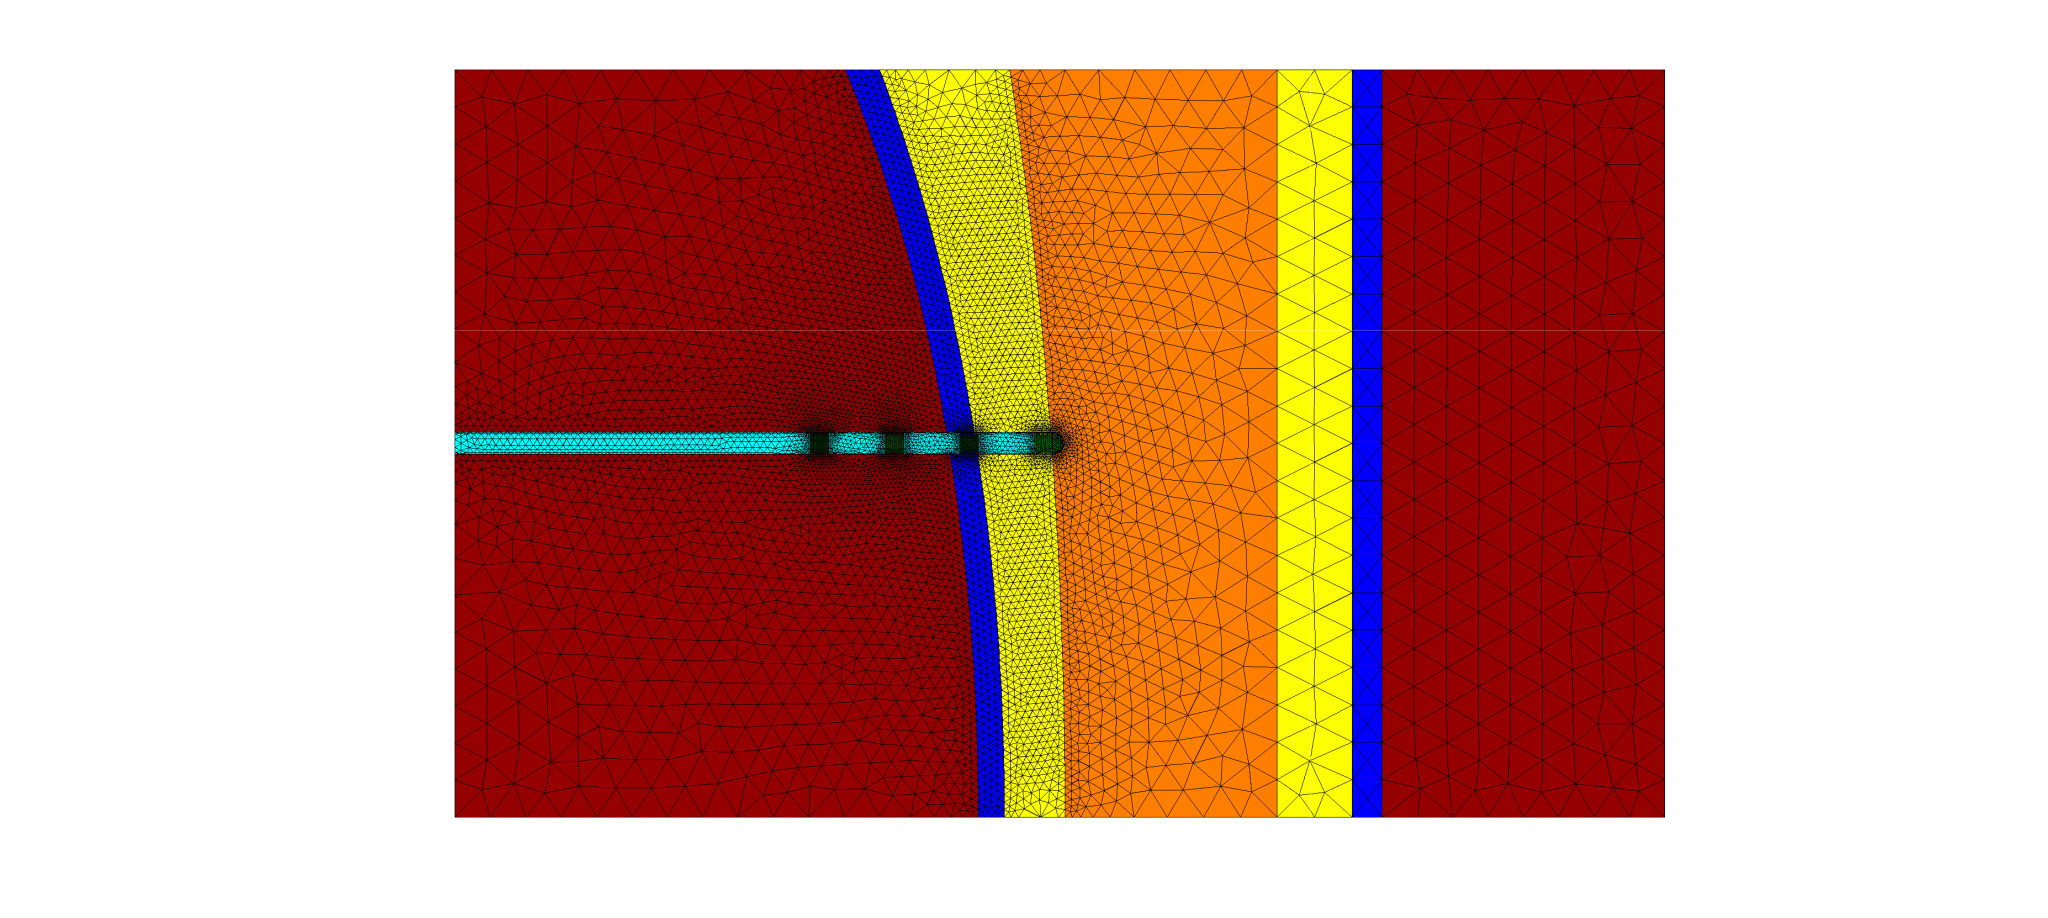
\includegraphics[width=0.50\columnwidth]{advanced_mesh.pdf}}\hfill
    \subfloat{
    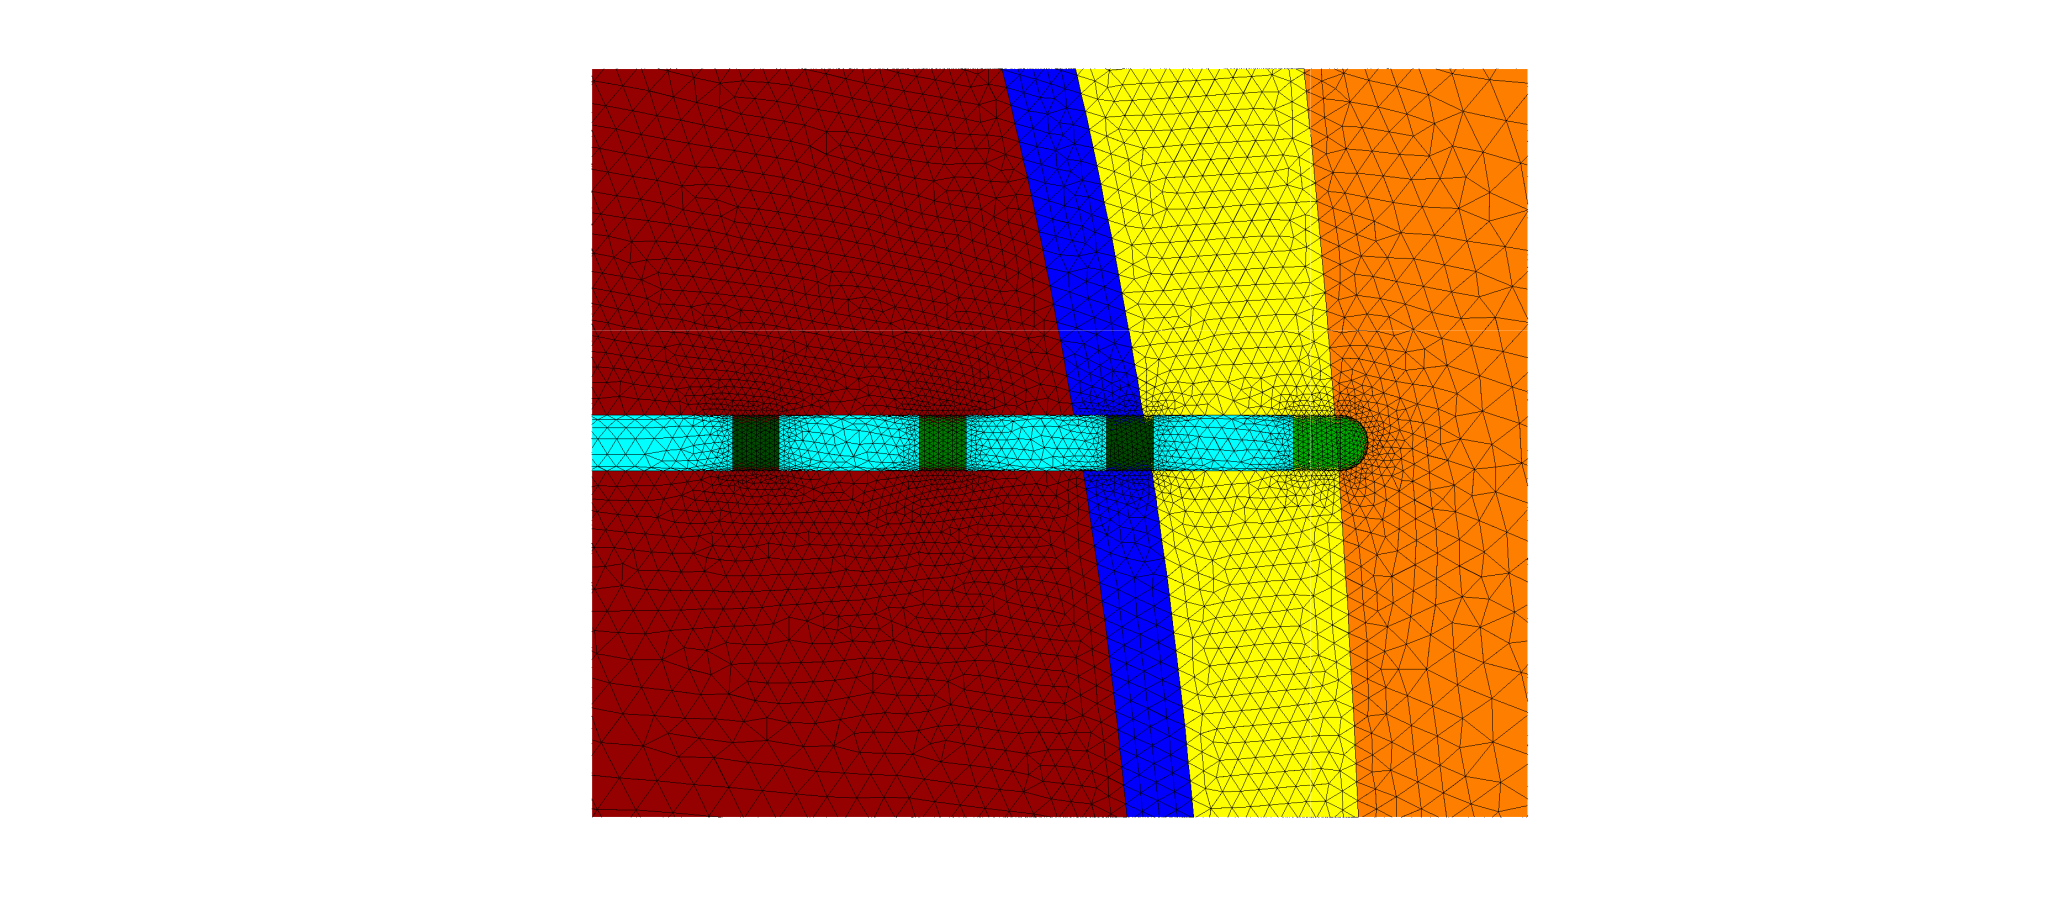
\includegraphics[width=0.705\columnwidth]{advanced_mesh_zoom.pdf}}
  %   \subfloat{
  %   \includegraphics[width=\columnwidth]{simulation_error}}
    \caption{\label{fig:adv_mesh} Example FEMs of a probe entering a bone from the surrounding 
    tissue. Refinement is specified around the electrodes and tissue interfaces near the probe.
    {\COMMENT{FIX CROP (just make it one figure in matlab...)}}}
  \end{figure}
  
\section{Results}

% Table 
\begin{table}[]
\caption{\label{tab:mesh-table}Your caption.}
\begin{tabular}{p{1cm}p{0.5cm}p{1cm}p{1cm}|p{1.4cm}p{1.4cm}p{1cm}|p{1.3cm}p{1.3cm}p{1.3cm}p{1.3cm}}
\multicolumn{2}{l}{Mesh ID} & glbl. maxh [mm] & elec. maxh [mm] & \#~elem. & \#~nodes & \#~elec. elem. & minEL\textsuperscript{\emph{a}} [mm] & maxEL\textsuperscript{\emph{b}} [mm] & minEV\textsuperscript{\emph{c}} [mm\textsuperscript{3}] & maxEV\textsuperscript{\emph{d}} [mm\textsuperscript{3}]\\ \hline 
\multirow{2}{*}{M-01} &A & 16.67 & 16.67 & 31347 & 7095 & 22 & 9.80 & 49.45 & 254.76 & 6851.01\\ 
& B & 16.67 & 16.67 & 49210 & 9615 & 25 & 10.32 & 50.00 & 222.87 & 2898.59\\ 
\multirow{2}{*}{M-03} &A & 18.33 & 15.00 & 29639 & 6482 & 22 & 10.75 & 50.41 & 289.80 & 5826.14\\ 
& B & 18.33 & 15.00 & 49247 & 9680 & 40 & 7.36 & 37.11 & 172.78 & 2814.55\\ 
\multirow{2}{*}{M-05} &A & 18.33 & 13.33 & 29814 & 6589 & 28 & 9.39 & 49.91 & 162.26 & 5648.41\\ 
& B & 20.00 & 13.33 & 50749 & 9930 & 42 & 7.80 & 37.93 & 134.41 & 3233.59\\ 
\multirow{2}{*}{M-07} &A & 18.33 & 11.67 & 30581 & 6723 & 36 & 8.77 & 47.88 & 141.74 & 6252.36\\ 
& B & 21.67 & 11.67 & 53002 & 10429 & 60 & 6.17 & 40.84 & 63.22 & 4077.18\\ 
\multirow{2}{*}{M-09} &A & 18.33 & 10.00 & 30690 & 6755 & 42 & 7.86 & 49.18 & 115.45 & 5496.39\\ 
& B & 23.33 & 10.00 & 56237 & 11008 & 68 & 5.82 & 43.81 & 62.88 & 4962.89\\ 
\multirow{2}{*}{M-11} &A & 18.33 & 8.33 & 31575 & 7030 & 74 & 6.05 & 50.99 & 60.06 & 6086.88\\ 
& B & 26.67 & 8.33 & 55545 & 10886 & 96 & 5.51 & 49.72 & 36.84 & 7424.70\\ 
\multirow{2}{*}{M-13} &A & 20.00 & 6.67 & 28589 & 6447 & 92 & 4.65 & 51.85 & 20.68 & 6664.11\\ 
& B & 30.83 & 6.67 & 54993 & 10825 & 148 & 4.51 & 55.36 & 20.63 & 10453.90\\ 
\multirow{2}{*}{M-15} &A & 21.67 & 5.00 & 27775 & 6245 & 158 & 3.46 & 52.60 & 11.13 & 9097.30\\ 
& B & 36.67 & 5.00 & 55331 & 11000 & 250 & 3.51 & 61.66 & 7.99 & 15838.09\\ 
\multirow{2}{*}{M-17} &A & 30.00 & 3.33 & 39116 & 7590 & 320 & 1.75 & 72.83 & 1.13 & 23783.17\\ 
& B & 48.33 & 3.33 & 52947 & 10798 & 548 & 2.32 & 86.60 & 2.72 & 32287.34\\ \hline 
\multirow{2}{*}{REF} &A & 3.33 & 3.33 & 6661789 & 1173243 & 510 & 1.75 & 9.49 & 1.01 & 46.09\\ 
& B & 3.33 & 3.33 & 5871464 & 976558 & 554 & 2.10 & 7.59 & 1.58 & 21.65\\ 
\multicolumn{11}{c}{\emph{a}: minimum mesh edge length, \emph{b}: maximum mesh edge length}\\ 
\multicolumn{11}{c}{\emph{c}: minimum mesh element volume, \emph{d}: maximum mesh element volume}\\ 
\end{tabular}

\end{table}

The sensitivity compared across all mesh densities 

{\COMMENT{I could have controlled netgen density similarly to try and find the ideal dissipation\dots
The only thing unique to Gmsh is the ability to refine around the internal structures and electrodes
if the method of "balance point" and refinement is going to be this basic\dots}

Basically there is no point to the  original analysis - it just shows that there is refinement in 
}

 \begin{figure}
    %\includegraphics[width=\columnwidth]{measurement_error}
    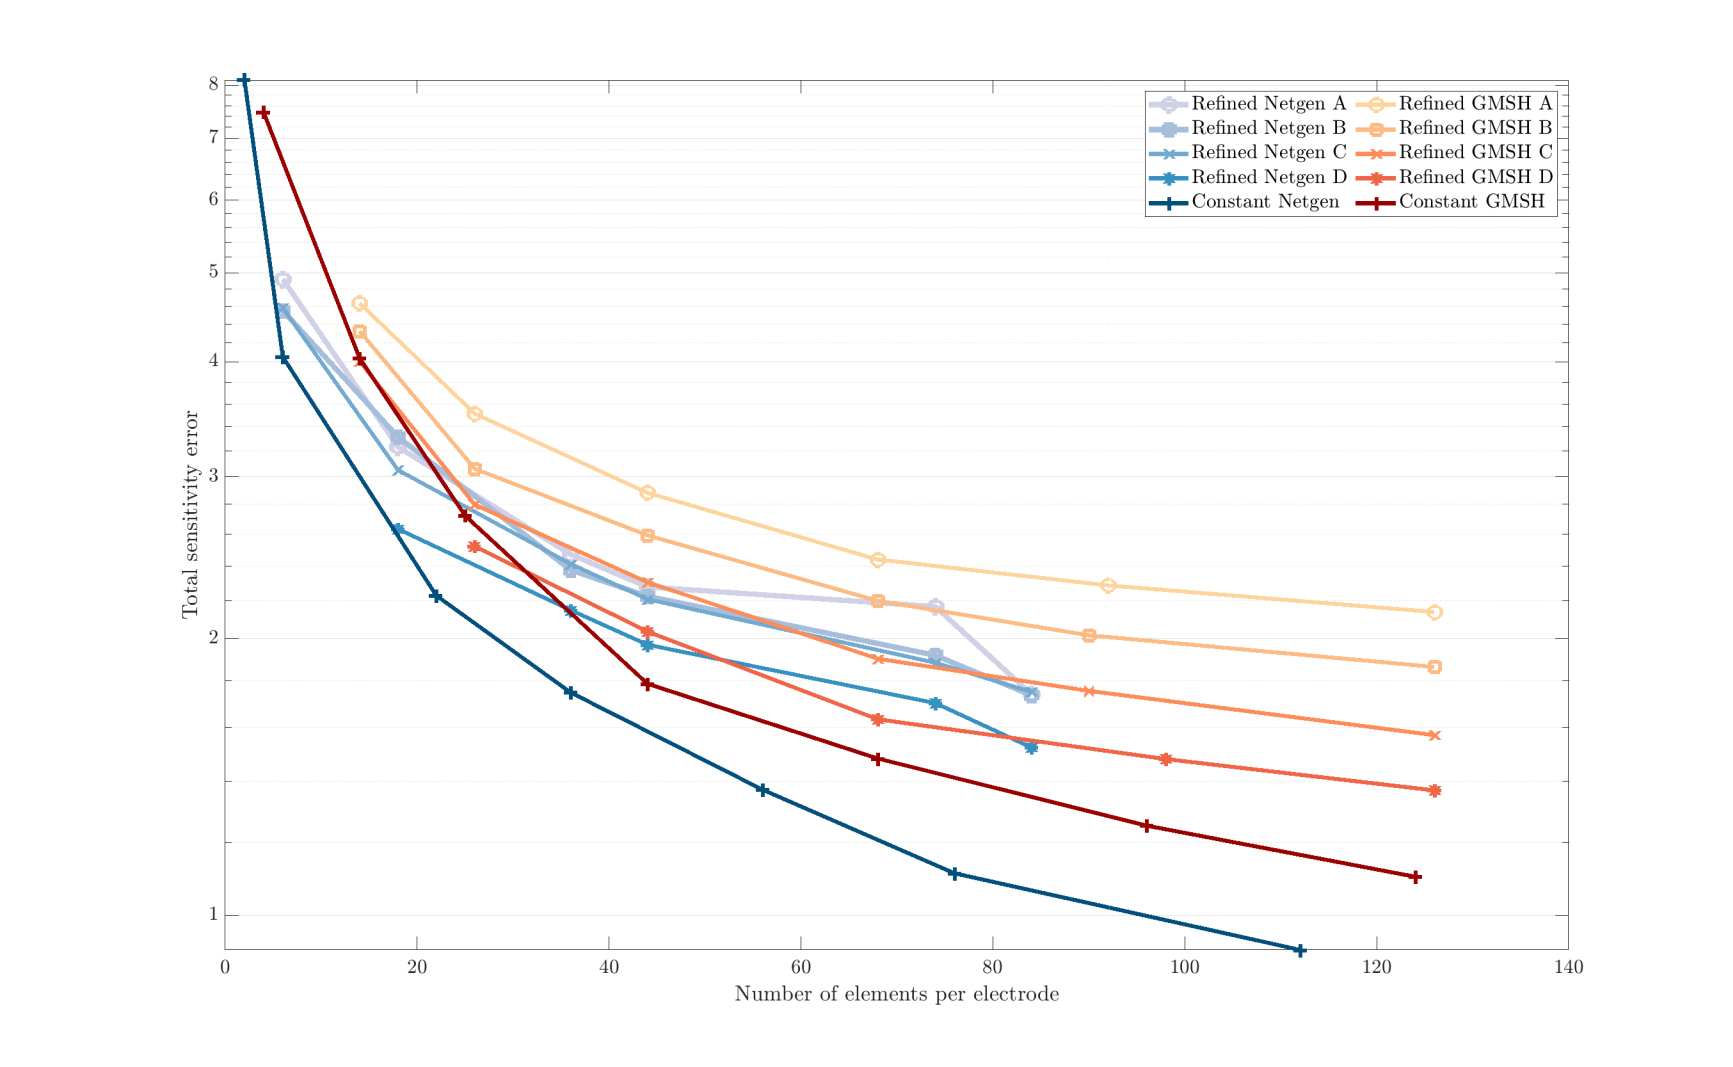
\includegraphics[width=\columnwidth]{sens_error_total.pdf}
    \caption{\label{fig:results_meas} Sensitivity error of each mesh as a function of the number of elements per electrode for both Netgen and Gmsh.
}
  \end{figure}
  
  Results show that for both Netgen and Gmsh there is a significant decrease in measurement error 
  as the number of elements throughout the model is increased. This is shown in Fig.~\ref{fig:results_meas} 
  where the measurement error on refined meshes decreases as the models are generated with a higher 
  density of elements. 
  
  For both Netgen and Gmsh when using mesh refinement techniques there was no change in the measurement error when compared to 
  the coarsest models. % THIS DOES NOT MATCH EARLIER RESULTS WHAT IS GOING ON NOW?!?!
  
  When comparing mech quality based on the average minimum angle in the tetrahedra, Netgen was shown to have a higher 
  quality mesh for constant models, but when using refinement Gmsh meshes had a better overall minimum angle score. 
  These results are presented in Fig.~\ref{fig:results_qual} 
  
   \begin{figure}
    %\includegraphics[width=\columnwidth]{mesh_quality}
    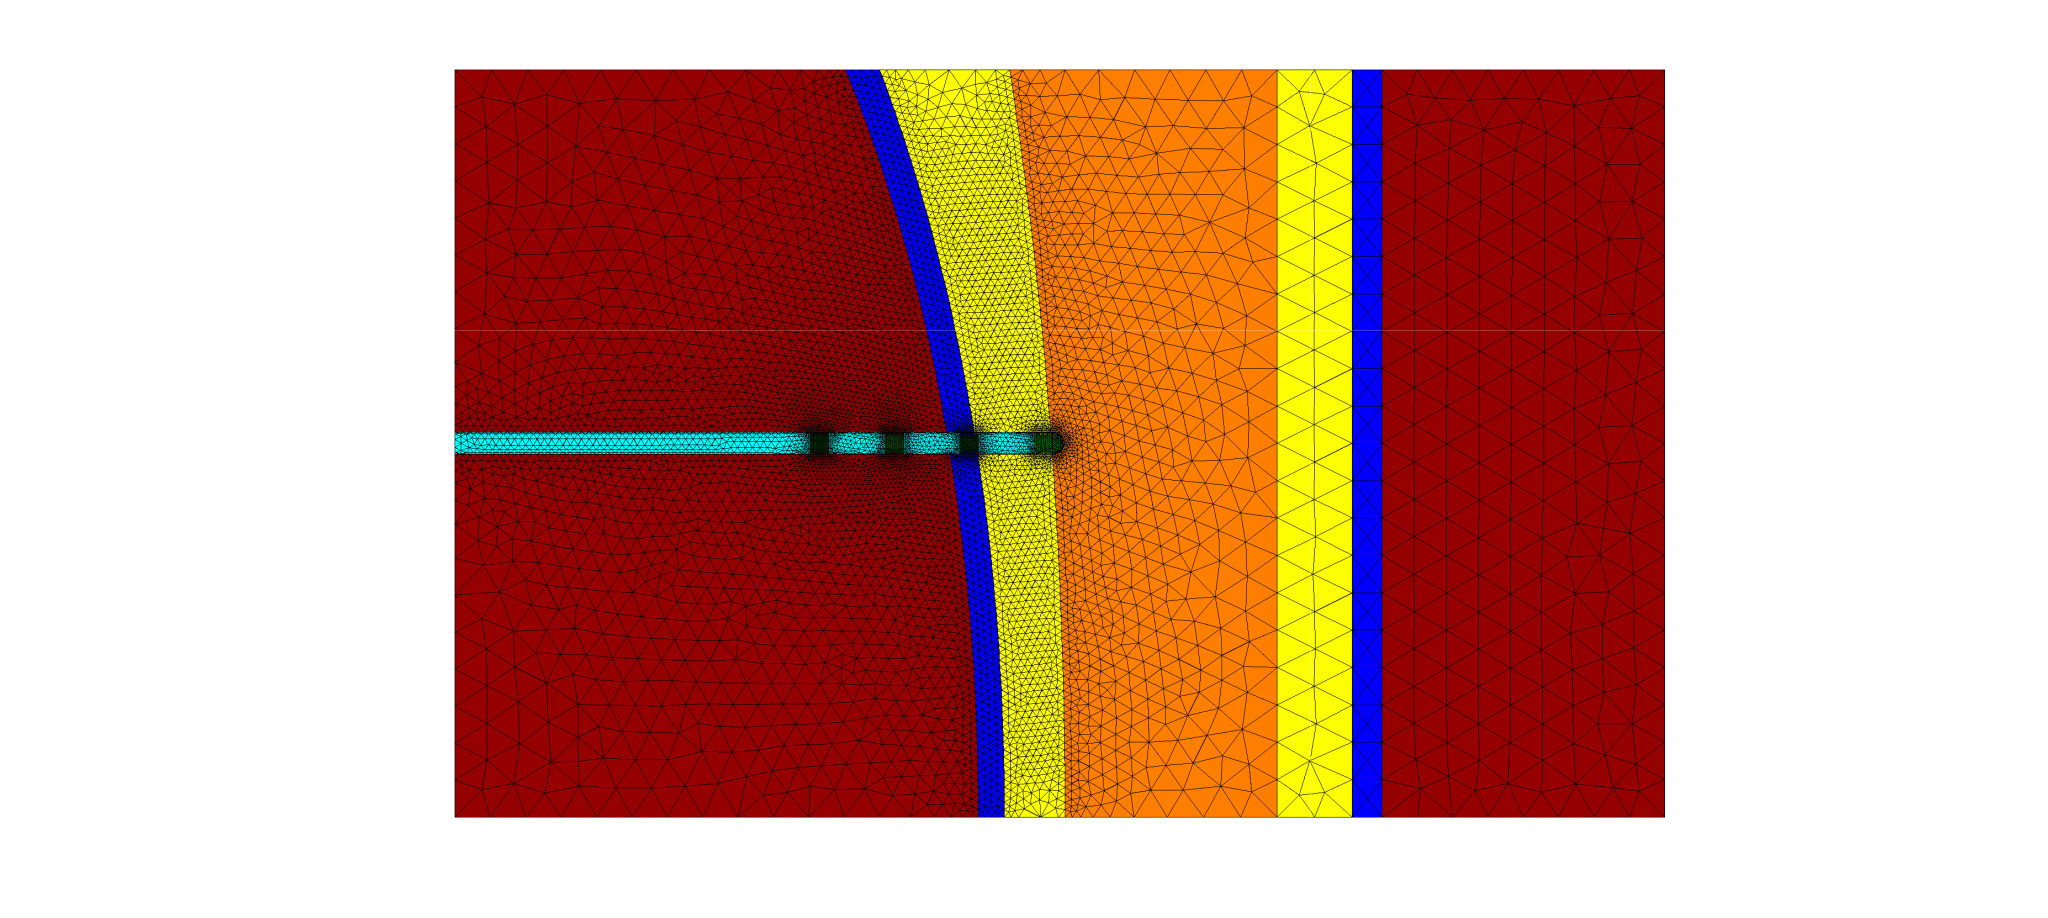
\includegraphics[width=\columnwidth]{advanced_mesh.pdf}
    \caption{\label{fig:results_original_} Mesh quality for each mesh as a function of the number of elements per electrode.}
  \end{figure}
  
  
  
\section{Discussion}
We consider the requirement of FEM refinement in the neighbourhood of
electrodes and the available tools for mesh refinement in EIT. 
While such refinement is generally agreed to be useful,
we have identified two problems: a lack of systematic analysis of
the required refinement level, and a difficulty in implementing and controlling such
refinement on arbitrary FE models. We present contributions in
both areas.

First, the benefit of electrode refinement has been analysed by considering
a sequence of refined FEMs compared to a ``gold standard", uniformly fine
FEM solution. The models were refined either globally or in the electrode
neighbourhood, and the voltage measurement,  and mesh quality %current distribution and sensitivity
were compared.

%Results are summarized in Fig.~\ref{fig:errors} which indicates
%that model errors near the electrodes decrease equally with electrode
Results are summarized in Fig.~\ref{fig:results_meas} which indicates
that Netgen had a much higher mesh quality for both constant and refined meshes 
when implementing mesh refinement 
coupled with a smaller number of elements per mesh at a specified 
mesh density. 
The results also indicated that despite the parameters used as input 
to specify mesh density with both programs, the result is not totally
controllable by the user. 

Despite the higher usability control by the user and option for refined mesh around both internal and
external electrodes the loss of quality and increase in measurement error when adapting the mesh density suggest 
that constant meshes of medium quality are the best balance between 
mesh quality and meshing speed. 
%that model errors near the electrodes decrease equally with electrode
%and uniform refinement. 
Errors away from the refined areas may be higher 
but with the ability to refine meshes selectively near regions where high sensitivity 
is required this may allow for reduced measurement error which still allowing for quicker 
meshing times.
%Model errors deeper in
%the body are improved with electrode refinement, but not as much as by
%uniform refinement (as would be expected). However, since errors deeper
%in the body are so much smaller, this may be less of a factor in many scenarios.
% Based on these results, we produced an additional model combining the electrode
% refinement of R8 and the maximum element size of C5 (18947 nodes and 98595
% elements). Its sensitivity
% error near the electrode was better than C2, while deeper in the medium it was
% on par with C5.  It produced measurement error of only 0.11~mV.

 
Additionally, we have developed a procedure to refine meshes on regions surrounding electrodes 
on internal and external surfaces on an arbitrary closed triangular surface mesh based exclusively on
open source software. 

To the best of the
authors' knowledge, no free pre-compiled tool exists to build meshes of
arbitrary geometries, as extracted e.g. from computed tomography (CT) data,
with controlled electrode refinement. Commercial FE modelling tools also do not offer an
easy interface to perform electrode refinement.
While our method combining two programs over whose results we do not have
full control is not without caveats, it addresses this important need in the
modelling community. 

\section{Conclusion}

In summary, as expected, refinement of electrode meshes near electrodes 
does improve model accuracy in terms of calculated voltage and sensitivity.
We recommend that, for each EIT imaging case, required model accuracy be
determined from an analysis of the system, and then the required electrode refinement 
be determined from Fig.\ \ref{fig:errors}. Additionally, we recommend that
a minimum of four FEM elements be used on any electrode model, to capture
the dynamics of current flow.
Further to these recommendations, by contributing freely available tools and 
tutorials for such electrode
refinement, we hope to facilitate such improved FE modeling in EIT.


  

  
 
\printbibliography

\end{document}
